%!TEX root = ../Peerbox.tex

As illustrated in Figure~\ref{fig:figures_archOverview} the Peerbox client is structured according to the layered approach. The Middleware-layer is concerned about low level network communication. The Logic layer provides the functionality for the VirtualFileSystem and contains the application logic. The UI represents the user layer and provides the functionality for user interaction.

\begin{figure}[htbp]
    \centering
        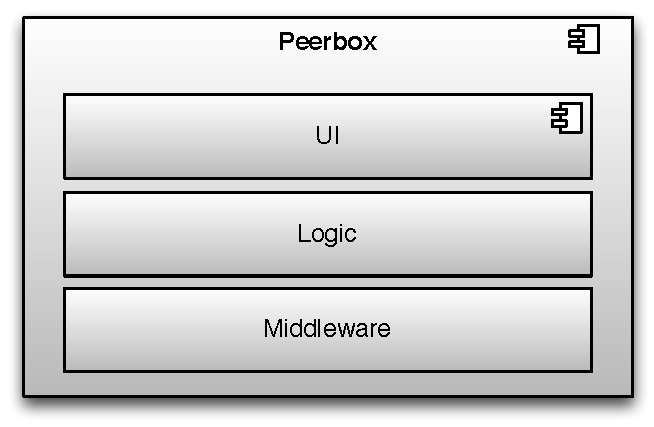
\includegraphics[height=2in]{figures/archOverview.pdf}
    \caption{Architectural overview}
    \label{fig:figures_archOverview}
\end{figure}

We have decided to use two different channels for communication. The general Peerbox related communication uses multicast message. while file transmission is implemented by using a 1-1 direct channel. 
The reason for that is that files are arbitrary large and would produce a lot of messages that need to be multicasted. Furthermore, not all clients might be interested in every file. Last but not least, a direct channel is fast and reliable as we can rely on the build-in properties of the TCP/IP protocol.

Peerbox has been implemented in Java 7 and uses the following third party libraries: 
\begin{itemize}
    \item Apache Commons Lang, for timed semaphore
    \item Apache Log4j, for general purpose logging
    \item Apache Commons IO, log file tailing
    \item SWT, user interface
\end{itemize}

\subsection{Middleware}

The middleware of peerbox uses IP-Multicast to announce messages to a group. However, basic multicast is not reliable and it does not ensure integrity, validity, agreement and ordering.

A test implementation of using the IP multicast showed a package loss of up to 20\% depending on the operating system, hardware and message frequency. 
Therefore, we need additional coordination and agreements on message receiving and delivery in form of a reliable multicast protocol.

% open vs. closed group 
%  only members can send to group, a member delivers to itself 
%  they are useful for coordination of groups of cooperating servers

The multicast protocol should ensure that all messages send to a group are eventually received and consumed by all process that are member of this group. Furthermore, messages need to be consumed in order, so that a file cannot be deleted before it has been created. 

For peerbox it is enough to ensure FIFO-ordering. Since a file always has a specific owner, it is enough if the messages from one process are consumed in order and independent from another process (no causality required). 

We implemented the reliable multicast based on the lecture slides, using  piggybacked messages number, negative acknowledgement and a holdback queue. Furthermore, we optimized the implementation using  multi-threading, bandwidth limiting, checksum and send optimizations. 
    



% % The IP address 224.0.0.0 through 239.255.255.255 are reserved for multicasts. The user needs to set some properties such as Path, Multicast address, Multicast port, Server Port and the name of the computer.
 
% over udp datagram
% 
% negative acknowledgements
% 
% reliable multicast
% 
% additional checksum to verify payload
% 
% Operations 
% multicast(g, m) sends message m to all members of process group g
% deliver (m) is called to get a multicast message delivered. It is different 
% from receive as it may be delayed to allow for ordering or reliability.

\subsubsection{Messages}
The basic entity of our reliable multicast implementation is a Message, which structure is shown in Figure~\ref{fig:messages}. The first byte represent the command, hence the message supports $2^8$ different commands. In our case, a command can be either Message (1), ACK(2) or NACK(4). However, ACK messages are not used in this implementation in order to reduce traffic on the channel. Furthermore, the peer and message number are represented each by four byte. Afterwards, the length of the payload is specified by two bytes. Eight bytes are reserved for the checksum, which is calculated on the payload. The actual payload has no fixed size and is only limited by the maximum message size, which is in our case is set to $2^{15}$.

\todo{CRC32 checksum} 

If the logic needs to send a lot of data, it has to be split into multiple messages. Due to the reliable multicast it is guaranteed that all messages will eventually arrive and are consumed in order.

\begin{figure}[htbp]
    \centering
        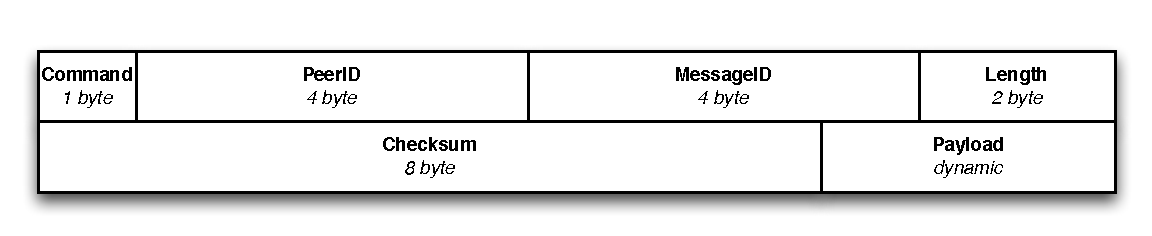
\includegraphics[width=.9\textwidth]{figures/message.pdf}
    \caption{Structure of a message}
    \label{fig:messages}
\end{figure}

\subsubsection{Delivering Messages form Group}

difference between receiving a message and delivering it

every process holds for every other process the id of the last consumed message and the id of the last seen message, ideally both are the same 

Figure~\ref{fig:figures_processReceivePackage} shows the process view on the activity of listeneing for incoming messages and processing those messages. the actual consumption and reliability process is shown in Figure~\ref{fig:figures_processMessages}.
The use of resources  is indicated by a dashed line 
processes are divided by swim-lanes (dotted vertical lines)
\begin{figure}[htbp]
    \centering
        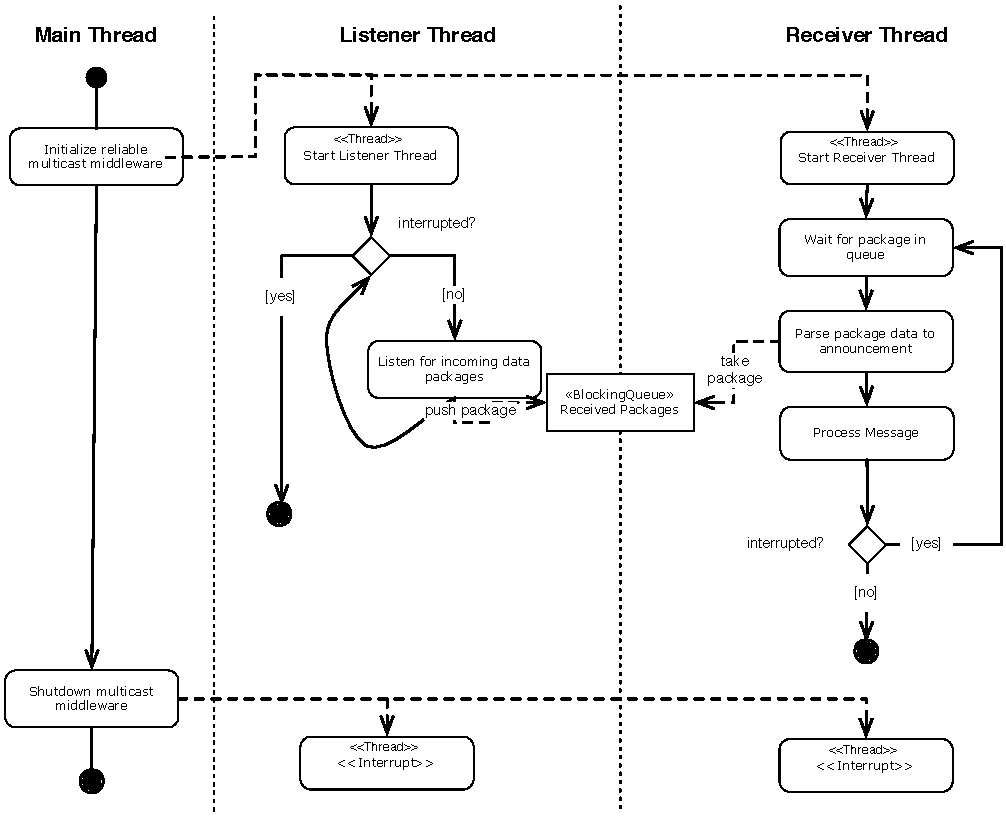
\includegraphics[height=4.5in]{figures/receivePackets.pdf}
    \caption{Listen for incoming multicast messages}
    \label{fig:figures_processReceivePackage}
\end{figure}
When the middleware is initialized it starts a separate listener threads and a received thread. The listener waits incoming messages on the channel of the multicast group. as soon as it receives a message, it pushes it on a blockingqueue for received packages and immediately continues to listen for the next message. 

Listening and processing of incoming messages has been decoupled by a blocking queue to decouple lengthy processing from receiving new messages, if the blocking queue is full, the listener thread has to wait until all packets have been processed. 

On the other side, the receiver thread takes packets from the blocking queue and processes them. if the queue is empty, it just waits until the listener thread has received and pushed the next package. 
At first the receiver thread parses the incoming packet into the aforementioned message structure and then decides wether the message is directly consumed, discarded or pushed on the holdback queue for later consumption.

this process is described in Figure~\ref{fig:figures_processMessages}.
Depending on the command of the message, the message either contains data or is a request for a missed message (Nack). If it is a NACK  then the process resends the message by taking it from the sent messages queue.

If the command is actually a message, it first checks wether it has ever received a message from that particularly process before. if not it initializes the piggyback counter and the seen message id to the id of the current message minus one. 
Afterwards, it compares the local piggybackcounter with the piggybacked messages number. One of three things might happen. 

1) The message has been seen before and is discarded
2) The message id is larger than the expected message, which means that a message has been missed. A negative acknowledge is send for the missed message. 
3) The message is expected and can be safely consumed.
 
\begin{figure}[htbp]
    \centering
        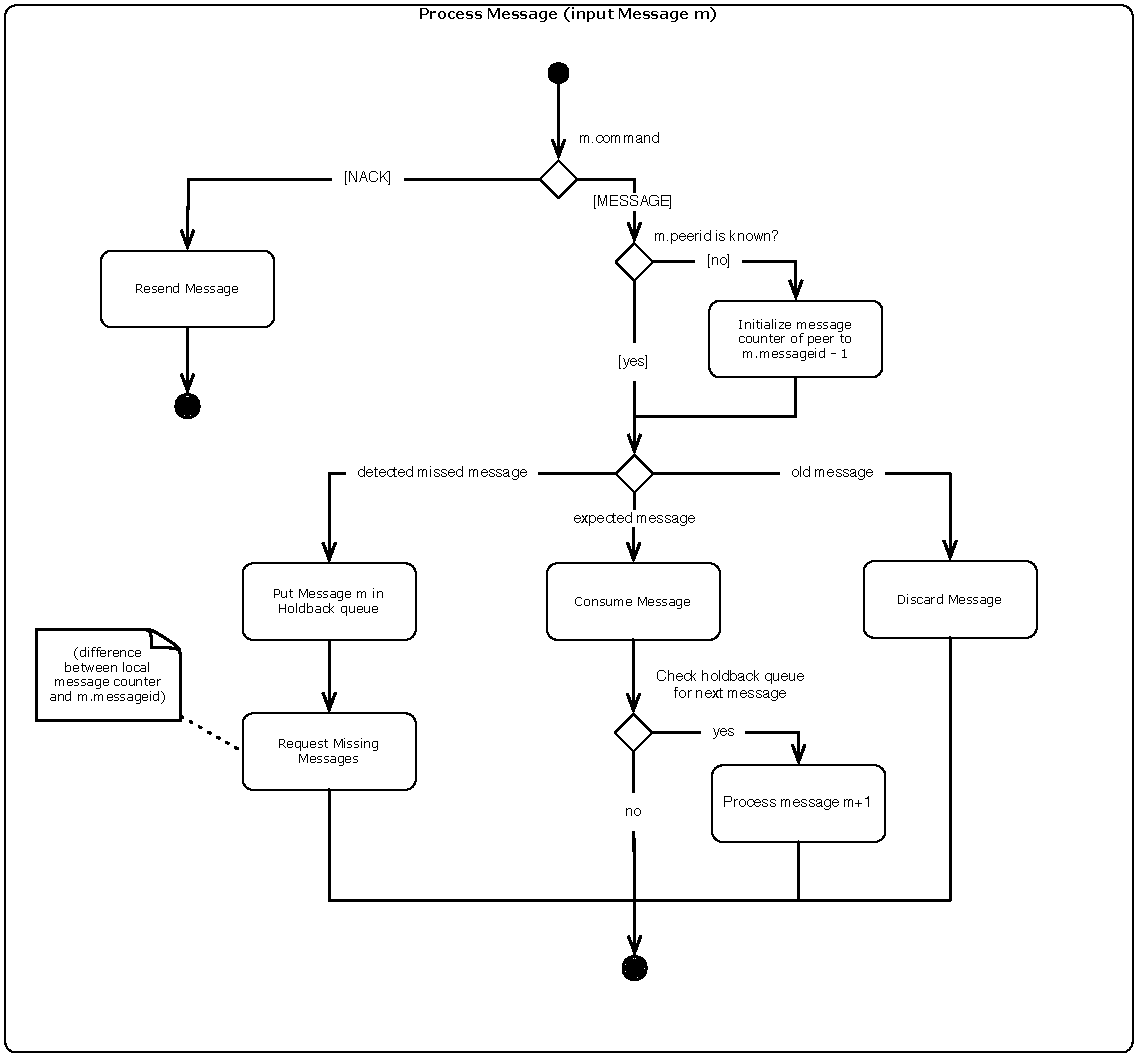
\includegraphics[height=4.5in]{figures/processMessages.pdf}
    \caption{Process incoming multicast messages}
    \label{fig:figures_processMessages}
\end{figure}

eventually delivers it

\subsubsection{Sending Messages to Group}

The process of multicasting a message to the group is described in Figure~\ref{fig:sendMessage}. Sending a message to a group is straightforward in Java. At first the message will be serialized into an array of bytes, which will be multicasted by using the Socket class. 

However, we have implemented various optimizations in order to improve reliability and avoid a clogging of the network. For instance, we figured out that if we limit the frequency of messages, less messages are lost. This is similar to limiting the bandwidth because less bits per seconds can be transferred.  
We implemented the limit by using a timed semaphore, which ensures that a critical path can only be entered every given time frame. Since Peerbox is not time critical it is no problem to limit the bandwidth. 
However, the timed semaphore is not enough because this will cause the application to halt until it can enter the critical section. Therefore, we decoupled  sending from the main application by using a blocking queue, which acts as a send buffer. 

In summary, the sender thread tries to acquire the semaphores, takes the next message from the queue, multicasts it to the group and then waits again for the semaphore and the next message. 

Furthermore, the send buffer allows to reduce the amount of sent messages by discarding messages that are already in the send buffer but were not yet multicasted to the group. Therefore, before pushing a message to the send buffer, it is checked if the message is already contained in the buffer.
An analysis of the network traffic showed that a lot of negative acknowledgements were sent multiple times because the process encountered a missed message multiple times but had not yet the chance to multicast the first negative acknowledgement. 

\begin{figure}[htbp]
    \centering
        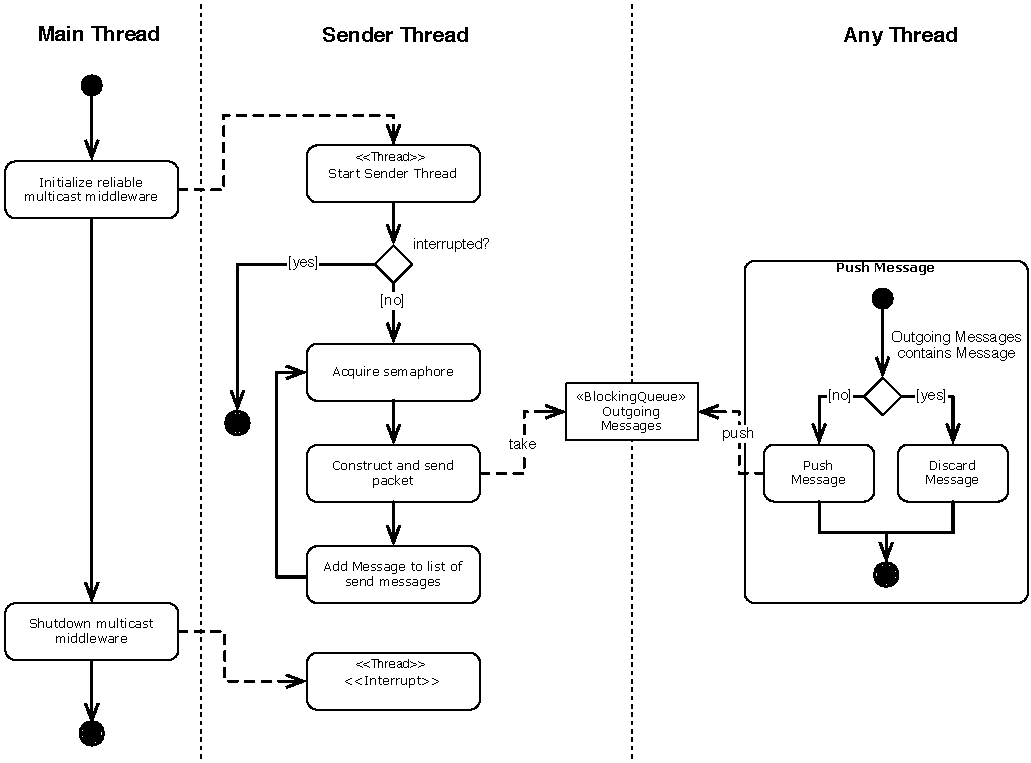
\includegraphics[height=3in]{figures/sendMessage.pdf}
    \caption{Send a multicast message}
    \label{fig:sendMessage}
\end{figure}
  
\subsubsection{Hearbeat}
A tough challenge is to handle peers that left without notice. Firstly, it is difficult to distinguish between a crashed peer or a slow peer and  secondly there is no automatic mechanism implemented in the basic multicast that informs other peers if a peer left the group.

We considered two tactics to increase fault-tolerance. The first one is a ping-echo tactic, in which a peer sends a ping message to another peer. If the peer answers with an echo message, everything is fine if not the peer is down for the count. We considered to implement the ping-echo mechanism using a reliable 1-1 channel, i.e. TCP/IP. In order to reduce the number of ping/echo messages, it would be good to have one peer that is responsible for sending out pings and detecting dead peers. This would require a leader-election algorithm.

The alternative is a heartbeat tactic, in which every peer multicasts a multicasts a life signal in a certain time interval. The dead peer detection is done by every peer on its own. Although the multicasted heartbeat might be less reliable as a fault-detection algorithm as it might happen that peers are in a different state (e.g. if one peer misses heartbeat messages), the complexity and total amount of messages is lower compared to the described ping/echo tactic.

Therefore we implemented a heartbeat mechanism into the middleware, to be able to detect unresponsive peers.

\subsubsection{Optimizations}
e
Miss Timer

easy to implement a vector clock in order to get partial ordering  (message may not be delivered until vector clock is as large)

limit bandwidth 
    - should be made dynamic
    
    , we favored a heartbeat over a ping tactic because we do not need to elect a leader for that. 
       every peer send a heartbeat every x second with its vector clock (showing its internal message state), if a peer 

       this might cause that a peer is temporarily not available also he is functioning properly.

\subsection{Logic}

The application logic is mainly responsible for processing dispatched messages from the middleware and maintain a consistent Virtual File System.
    
    \subsubsection{Messages}
    serialized dictionary
    dynamic structure realized by a serialized key-value store. 
    this allows to easily extend the protocol

    \subsubsection{Dynamicity}
    ip of peers is transmitted and thus dynamically discovered
    all options are configurable via configuration files
    no hardcoded properties
    works on any ip network that support multicast
    
    
    \subsubsection{Message handling}
    Strategy pattern, depending on the Key.Command the appropriate handler will be chosen.
    
    \subsubsection{VirtualFileSystem}
    
    observe folder changes
    
    associate files with peers
    
    limitation: no real fs, hence it is possible to invalidate the state of the vfs by modifying the folder when the application is not running. 
    
    \subsubsection{Requesting a file}
    
    direct communication, multicasting files might be inappropriate
    

    
    
    

\subsection{Interface}